\documentclass[12pt]{article}
%\documentclass[12pt,legalpaper]{article}
%\documentclass[14pt,legalpaper]{extarticle}
\usepackage{fullpage}
\usepackage{amsmath,amssymb}
\usepackage{mathptmx}
\usepackage{fancyhdr}
\usepackage{lastpage}
\usepackage{multicol}
\usepackage{graphicx}
\usepackage[aux]{rerunfilecheck}
\usepackage[rflt]{floatflt}

%\setlength{\textheight}{11.5in}

\reversemarginpar

\newcommand{\myimp}{\Rightarrow}
\newcommand{\myiff}{\Leftrightarrow}
\newcommand{\mynot}{\neg}
\newcommand{\myor}{\vee}
\newcommand{\myand}{\wedge}
\newcommand{\ds}{\displaystyle}

\DeclareSymbolFont{AMSb}{U}{msb}{m}{n}
\DeclareMathSymbol{\N}{\mathbin}{AMSb}{"4E}
\DeclareMathSymbol{\Z}{\mathbin}{AMSb}{"5A}
\DeclareMathSymbol{\R}{\mathbin}{AMSb}{"52}
\DeclareMathSymbol{\Q}{\mathbin}{AMSb}{"51}
\DeclareMathSymbol{\I}{\mathbin}{AMSb}{"49}
\DeclareMathSymbol{\C}{\mathbin}{AMSb}{"43}

\pagestyle{fancy}
\lhead{MATH 110 200930                                                     \\ 
  Sample Final Examination 1 \hspace{0.75in} Page\ \thepage\ of \pageref{LastPage}  \\ 
  Time: 3 hours                                                            \\
  \quad                                                                      }
%\chead{\quad                                                              \\ 
%       Page\ \thepage\ of \pageref{LastPage}                              \\ 
%	\quad                                                                }
\chead{}
\rhead{Name: \underline{\hspace{2in}}        \\ 
       Student \#: \underline{\hspace{2in}}  \\ 
       Section: \underline{\hspace{2in}}     \\
       \quad                                   }
\cfoot{}
\addtolength{\headheight}{\baselineskip}
\addtolength{\headheight}{\baselineskip}
\addtolength{\headheight}{\baselineskip}
\addtolength{\headheight}{\baselineskip}
\renewcommand{\headrulewidth}{0pt}
\fancypagestyle{plain}{%
  \lhead{}
  \chead{FIRST NATIONS UNIVERSITY OF CANADA                \\
    DEPARTMENT OF SCIENCE \\
    MATH 110 200930 \\
  }
  \rhead{}
  \cfoot{Page\ \thepage\ of \pageref{LastPage}}
}

\title{Sample Final Examination 1}
\author{Edward Doolittle, Martin Argerami, Sergei Panafidin, Richard McIntosh, Fotini Labropulu, L.\ Dame}

\begin{document}
\thispagestyle{plain}
%\maketitle

\begin{center}
  \LARGE{MATH 110 200930 Sample Final Examination 1}
\end{center}

\begin{flushleft}
\quad\\
Time:  3 hours                  \hfill       Name: \underline{\hspace{2in}}  \\
Instructors:                    \hfill Student \#: \underline{\hspace{2in}}  \\
\quad Dr. Edward Doolittle      \hfill    Section: \underline{\hspace{2in}}  \\
\end{flushleft}


\noindent
You have 3 hours to do each of the following questions.
The test is worth a total of 100 marks.
Please\marginpar{\footnotesize{(marks)}} justify your conclusions and
show all your work.
A non-programmable calculator of the type mentioned in the course outline
is permitted; no other aids are permitted.
%Use the backs of the pages for rough work.

\begin{enumerate}
\item Find\marginpar{\footnotesize{(10)}}
  an equation of the tangent line to the curve $(x^2+y^2)^2=2(x^3+y^2)$
  at the point $(1,1)$.
\newpage
\item Evaluate\marginpar{\footnotesize{(15)}}
  the following limits if they exist.
  \begin{enumerate}
  \item $\ds \lim_{x\to 2} 
    \frac{x^2+4x+3}{x^2+6x+5}$
\vfill
  \item $\ds \lim_{x\to -1} \frac{x^2+4x+3}{x^2+6x+5}$
\vfill
  \item $\ds \lim_{x\to\infty} \frac{2x^2-1}{3x^2+x+2}$
\vfill
  \item $\ds \lim_{h\to 0} \frac{\sqrt{4+h}-2}{h}$
\vfill
  \item $\ds \lim_{x\to 0} \frac{1-\cos x}{x\sin x}$
\vfill
  \end{enumerate}
\newpage
  \begin{center}
    \includegraphics[width=6in]{grph.eps}%
  \end{center}
\item Consider\marginpar{\footnotesize{(6)}} 
  the above graph of the function $g$.
  \begin{enumerate}
  \item Determine all real numbers $x$ where $g$ is not differentiable.
\vfill
  \item List all open intervals on which $g$ is continuous.
\vfill
  \end{enumerate}
\newpage
\item Find\marginpar{\footnotesize{(6)}} 
  the value of the constant $b$ that makes the following function
  continuous.
  \begin{align*}
    f(x) = \begin{cases}
      2x+b       & \mbox{if $x<0$}    \\
      \sqrt{x+4} & \mbox{if $x\ge 0$}
    \end{cases}
  \end{align*}
\vfill
\item A\marginpar{\footnotesize{(10)}}
  ladder $20$ ft long leans against a building.  If the bottom of the
  ladder slides away from the building horizontally at a rate of $2$ ft/sec,
  at what rate is the angle between the ladder and the ground decreasing
  when the top of the ladder is $12$ ft above the ground?
\vfill
\vfill
\newpage
\item Find\marginpar{\footnotesize{(10)}} 
  $\ds \frac{dy}{dx}$ in each of the following cases.  (You do not have to
  simplify your answers.)
  \begin{enumerate}
  \item $\ds y=x^9 + \frac{\sqrt[9]{x}}{2} + \tan x$
\vfill
  \item $\ds y = (3x+7)^8 (4x^2-9x)^5$
\vfill
  \item $\ds y = \frac{\sin^3(2x)}{x^2+x+9}$
\vfill
  \item $\ds 2x^2+4xy+3y^2=9$
\vfill
  \end{enumerate}
\newpage
\item Let\marginpar{\footnotesize{(10)}}
  $\ds f(x)=\sqrt[3]{(x^2-1)^2}$.  Then
  $\ds f'(x) = \frac{4x}{3\sqrt[3]{x^2-1}}$ and
  $\ds f''(x) = \frac{4(x^2-3)}{9(x^2-1)^{4/3}}$.
  \begin{enumerate}
  \item Identify all (if any) \\
    local maxima \hrulefill \\
    local minima \hrulefill \\
    points of inflection \hrulefill \\
    asymptotes \hrulefill 
  \item Determine the intervals on which $f$ is \\
    increasing \hrulefill \\
    decreasing \hrulefill \\
    concave up \hrulefill \\
    concave down \hrulefill
  \item Use the above information to sketch a graph of $f$.  If more space
    is required, use the back of the facing page and indicate that you have
    done so.
\vfill
  \end{enumerate}
\newpage
\item An\marginpar{\footnotesize{(10)}} 
  athletic field consists of a rectangular region with a semicircular region
  at each end.  The perimeter will be used for a $400$ m track.  Find the
  dimensions that maximize the area of the rectangular region.
\vfill
\item Draw\marginpar{\footnotesize{(10)}}
  the region bounded by $y=\sin x$, $y=\cos x$, and bounded on the left by
  the $y$-axis.  Calculate the area of this region.
\vfill
\newpage
\item Evaluate\marginpar{\footnotesize{(13)}} 
  the following integrals.
  \begin{enumerate}
  \item $\ds \int \frac{(t^2+1)^2}{t^2} \; dt$
\vfill
  \item $\ds \int x \sqrt[3]{x+1} \; dx$
\vfill
  \item $\ds \int 4x^3 \; \cos(x^4+1) \; dx$
\vfill
  \item $\ds \int_0^{\pi/2} (\cos x) \sqrt{3+5\sin x} \; dx$
\vfill
  \end{enumerate}
\end{enumerate}
\end{document}

